% !TEX encoding = UTF-8
% !TEX TS-program = pdflatex
% !TEX root = ../tesi.tex

%**************************************************************
\chapter{Container VS Virtual Machine}
\label{cap:container-vm}
%**************************************************************

\intro{Introduzione al capitolo}\\
Nel presente capitolo si esporranno le principali differenze tra un'architettura basata su macchine virtuali ed un'altra basata invece su container, analizzando i pro ed i contro di entrambe le architetture e fornendo al lettore una panoramica sulla tecnologia di containerizzazione utilizzata in ambito aziendale.

%**************************************************************
\section{Differenze architetturali tra Container e VM}
La \textbf{virtualizzazione} è un insieme di software in grado di astrarre componenti \gls{hardwareg}, permettendo l'esecuzione, anche simultanea, di più \gls{sistemi operativig} su un singolo \gls{clientg}. Verso la fine degli anni '90, la virtualizzazione ha cominciato ad essere sempre più utilizzata in ambienti \textit{enterprise}, permettendo un aumento di scalabilità e flessibilità dell'infrastruttura informatica aziendale riducendone notevolmente i costi di gestione\footcite{fonte: https://www.vmware.com/it/solutions/virtualization.html}. I \textbf{vantaggi} legati all'utilizzo della virtualizzazione, nello specifico, tramite l'uso di una o più macchine virtuali, comportano una separazione tra il sistema operativo \gls{hostg} e \gls{guestg}, fornendo una serie di accessi logici utilizzati da utenti esterni agli applicativi eseguiti in ogni macchina virtuale. \\
Oltre ad una esecuzione parallela, dal punto di vista dell' \textit{host}, un'architettura a VM è più facilmente \textbf{manutenibile}: una macchina virtuale infatti, può essere facilmente aggiornata, avviata o arrestata in base alle esigenze di carico (ex: \textit{\gls{load-balancingg}}) o aziendali.
La virtualizzazione, inoltre, aumenta l'\textbf{affidabilità} dell'intero sistema, in quanto garantisce l'\textbf{isolamento} di programmi e servizi i quali non andranno in conflitto tra di loro, contenendo, in aggiunta, il numero di server fisici presenti in \gls{datacenterg} nel caso in cui molteplici macchine virtuali vengano eseguite su un singolo \textit{host}, con conseguente notevole riduzione dei costi legati all'hardware.\\
Un ulteriore vantaggio della virtualizzazione si rivela in caso di \textit{\gls{disaster recoveryg}}, dove l'intero sistema operativo \textit{guest} può essere facilmente ripristinato su un altro server, indipendentemente dall'\textit{hardware}, riducendo così notevolmente i tempi di indisponibilità di servizio (\textit{downtime})  favorendo una più facile e rapida procedura di data \textit{\gls{recoveryg}}.\\
Esistono diversi tipi di virtualizzazione: \textbf{\textit{native}} e \textbf{\textit{hosted}}.
Una virtualizzazione di tipo \textbf{native} si appoggia all'\textit{hardware} \textit{host}, controllandolo direttamente per garantire tutte le funzionalità della virtualizzazione. Un esempio di applicativo dedicato alla virtualizzazione di tipo \textit{hosted} può essere, ad esempio, \textbf{\gls{Hyper-Vg}} della Microsoft\footcite{questa funzionalita' e' presente solamente nelle versioni Pro e Server di Windows 10} oppure l'applicativo \textbf{\gls{Xeng}} ampiamente utilizzato anche nell'ambiente Cloud di Amazon.
La virtualizzazione di tipo \textbf{hosted} è invece in esecuzione sul sistema operativo \textit{host} senza alcuna interfaccia diretta con l'hardware del computer. Questo tipo di virtualizzazione è molto diffusa, in quanto permette di accedere, in una maniera semplice ed immediata, al sistema operativo \textit{host} e \textit{guest} simultaneamente. Gli applicativi più usati in ambito \textbf{enterprise} che usano un tipo di virtualizzazione \textit{hosted} sono, ad esempio, \textit{VMware} o il gratuito \textit{VirtualBox}.\\
%TODO: Esempio di Windows 10 Pro virtualizzato tramite Hyper-V
Nella seguente figura è rappresentato il sistema operativo Windows 10 Pro virtualizzato con in esecuzione il browser web "Mozilla Firefox" tramite le due soluzioni software di virtualizzazione \textit{hosted} appena descritte:
\begin{figure}[!h]     
\centering 
    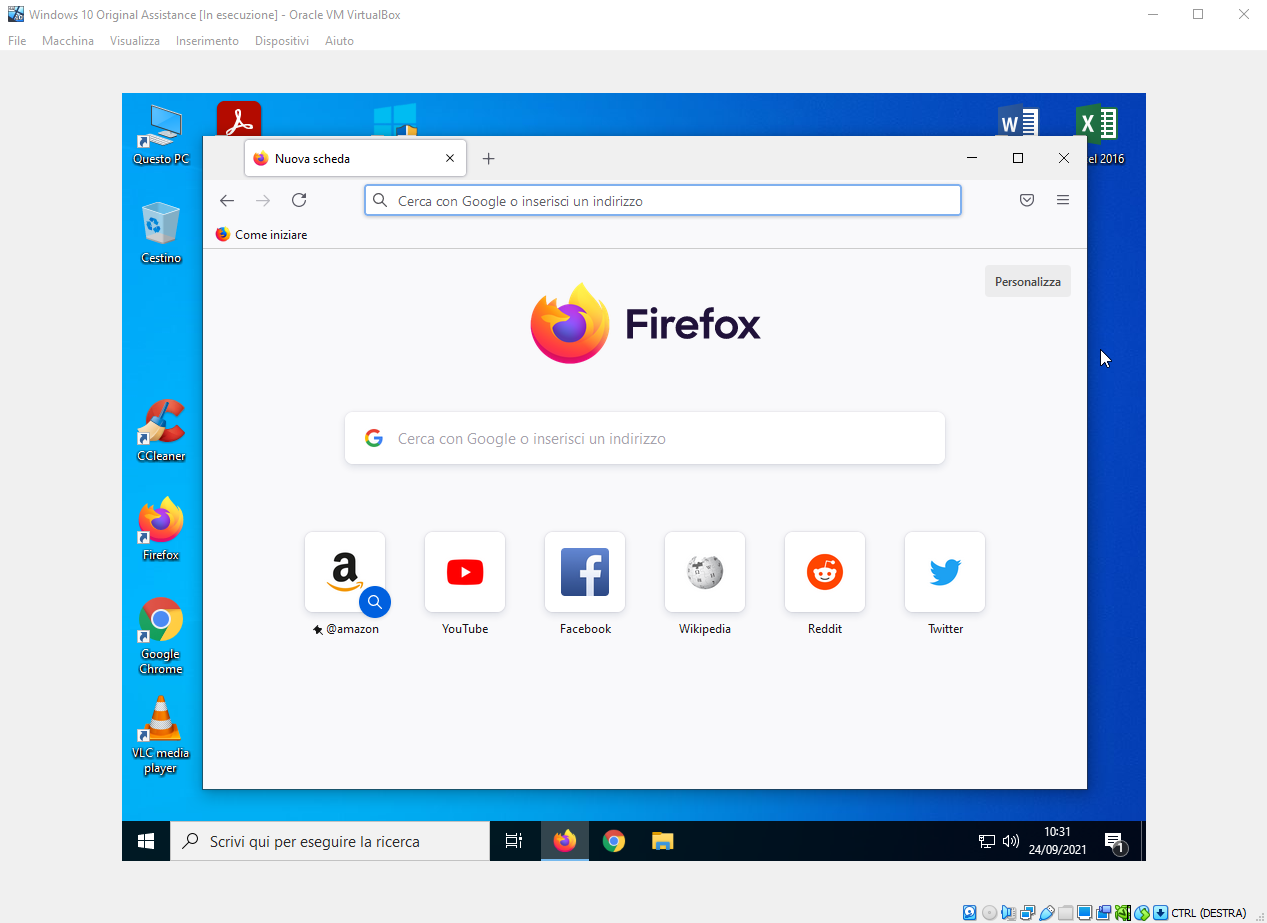
\includegraphics[width=0.6\columnwidth]{immagini/screenshot/firefox_virtualbox} 
    \caption{Browser "Firefox" virtualizzato tramite software di virtualizzazione "VirtualBox"}
\end{figure} \\

\begin{figure}[!h]     
\centering 
    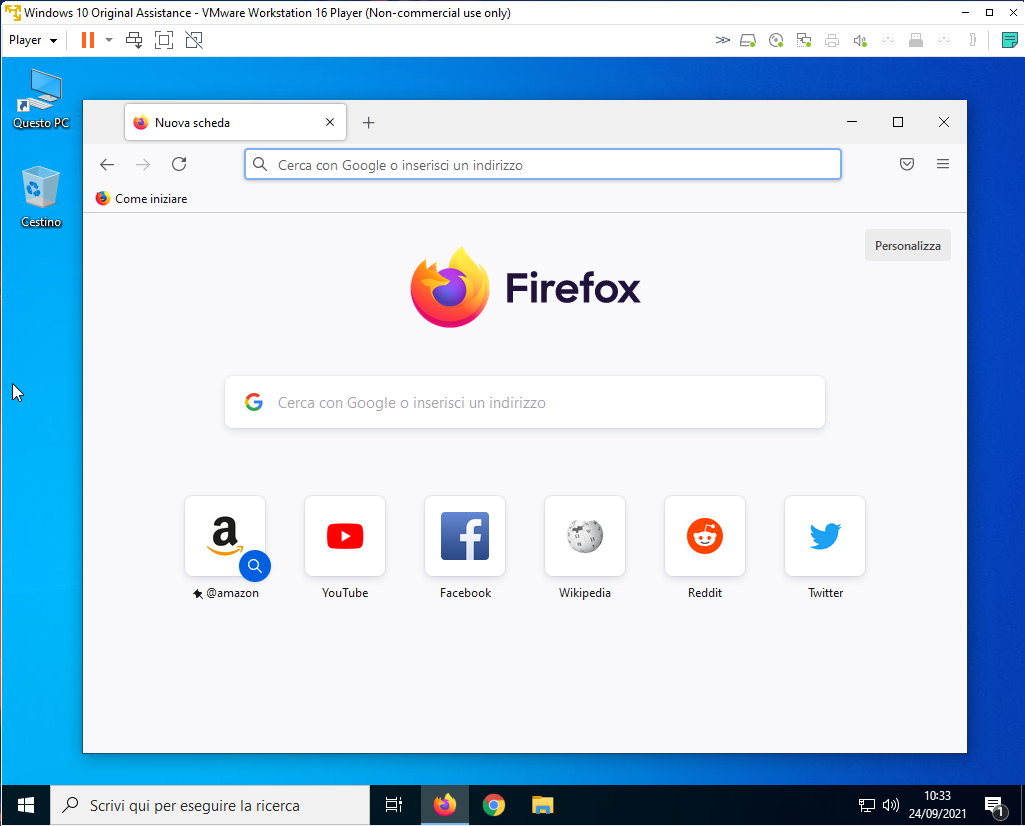
\includegraphics[width=0.6\columnwidth]{immagini/screenshot/firefox_vmware} 
    \caption{Browser "Firefox" virtualizzato tramite software di virtualizzazione "VMWare"}
\end{figure}
\newpage

Al fine di permettere al sistema operativo \textit{host} la virtualizzazione di uno o più sistemi operativi, è necessario installare un \textit{\gls{hypervisorg}}\footcite{installabile solamente se il processore supporta la virtualizzazione e se quest'ultima e' abilitata da BIOS}, \textit{native} o \textit{hosted}, ovvero uno strato software che si interfacci e gestisca tutte le \textbf{istanze} di macchine virtuali in esecuzione sulla macchina locale. \\
La virtualizzazione non è priva di svantaggi. Il primo tra tutti, è appunto la necessità di dover \textit{virtualizzare} un intero sistema operativo al fine di eseguire l'applicativo virtuale desiderato.
Questo vincolo obbligatorio implica un consumo di memoria \gls{RAMg} e di \gls{storageg} non indifferente anche solo per eseguire il singolo sistema operativo virtualizzato \textbf{senza alcuna} applicazione virtuale in esecuzione.
Ne consegue quindi, che un'architettura a macchine virtuali avrà bisogno di uno spazio di \textit{storage} e di un quantitativo di memoria \textit{RAM}\footcite{il tipo di RAM "ECC" risulta preferibile ma non obbligatorio} installata sul server non indifferente. Anche in termini di consumo \textit{\gls{CPUg}}, la virtualizzazione di molteplici sistemi operativi con le relative applicazioni virtualizzate in esecuzione può comportare \textbf{grossi carichi prestazionali} al server fisico, in quanto la CPU dell'host dovrà servire ed eseguire ogni sistema operativo di \textbf{ogni istanza} di virtualizzazione.\\
Dal punto di vista della sicurezza, quando si virtualizza un sistema operativo, sia nella virtualizzazione \textit{native} che \textit{hosted}, alcuni registri CPU sono direttamente esposti alla macchina virtuale come, ad esempio, i registri \textbf{VT-x} e \textbf{VT-d} del processore\footcite{e' necessario abilitare le estensioni di virtualizzazione da BIOS della scheda madre.} \footcite{nel caso di architettura avente processori Intel, IOMMU per architetture basate su processori AMD.}. Questi registri permettono al processore di non rendere accessibile la totalità dei suoi registri all'\textbf{hypervisor} e di controllare le chiamate dirette al \textit{\gls{DMAg}} da parte delle soluzioni software virtualizzate.\\
Relativamente alla condivisione della rete tra macchine virtuali e host fisico, nel caso in cui si fosse installato un commutatore di rete virtuale di tipo \textbf{\gls{NATg}}, la scheda di rete dell'host e il relativo traffico sarebbe \textbf{esposta} a tutto il set applicativo virtualizzato e viceversa, con conseguente mancanza di isolamento tra macchine virtuali stesse ed \textit{host} fisico. Ne conseguirebbe quindi, che eventuali condivisioni di rete, o connessioni applicative, sarebbero disponibili a \textbf{tutto il set} di macchine virtuali. \\
Una possibile soluzione a questo problema potrebbe essere il passaggio da commutatore virtuale di tipo \textit{NAT} ad un commutatore virtuale che riesca ad isolare le singole macchine virtuali tra di esse e l'\textit{host} fisico, anche, nel caso più estremo, assegnando ad ogni macchina virtuale una \textbf{propria scheda di rete} ed una \textbf{propria} \textit{\gls{VLANg}} di rete dedicata\footcite{per creare o impostare una VLAN, fare riferimento al router/firewall o allo switch di rete}.\\
Virtualizzare un intero sistema operativo implica, come abbiamo appena analizzato, un \textbf{elevato consumo di risorse fisiche}, specialmente nel caso in cui, per esigenze lavorative, si debba ricorrere ad una multipla virtualizzazione di sistemi operativi dove, in ognuno di essi, viene eseguita una specifica applicazione che deve essere accessibile ad altri \textit{client}.\\
Uno dei principali aspetti positivi di un'architettura a container sta proprio nel poter virtualizzare (o \textit{containerizzare} nel caso appunto di container) una singola e specifica applicazione \textbf{senza la necessità di inglobare un intero sistema operativo} nell'immagine virtuale. L'esecuzione dell'applicativo, nonostante appunto la mancanza di un sistema operativo, sarà comunque possibile grazie a chiamate di sistema al kernel del sistema operativo \textit{host}. Ne consegue quindi, che il container applicativo risultante di un'applicazione \textit{containerizzata} è di gran lunga di \textbf{dimensione inferiore} rispetto all' immagine\footcite{inteso come dimensione in Gb del virtual disk image (*.vdi) dell'immagine virtualizzata} della stessa applicazione \textit{virtualizzata}, causa appunto, in primis, mancanza di sistema operativo.\\
Un container è quindi una \textbf{singola unità atomica} contenente l'applicativo (il programma \textit{containerizzato}) con i relativi file atti alla sua corretta esecuzione senza l'immagine di un sistema operativo completo.
Al momento dell'esecuzione del container, l'applicazione \textit{containerizzata} verrà eseguita immediatamente sopra lo stato del sistema operativo \textit{host}, attraverso l'aiuto del \textbf{\gls{Docker Engineg}}, senza alcun \textit{\gls{hypervisorg}} come, ad esempio, nel caso dell'architettura a macchine virtuali. \\
Una rappresentazione grafica del concetto appena descritto è data dalla seguente immagine:
\begin{figure}[!h]     
\centering 
    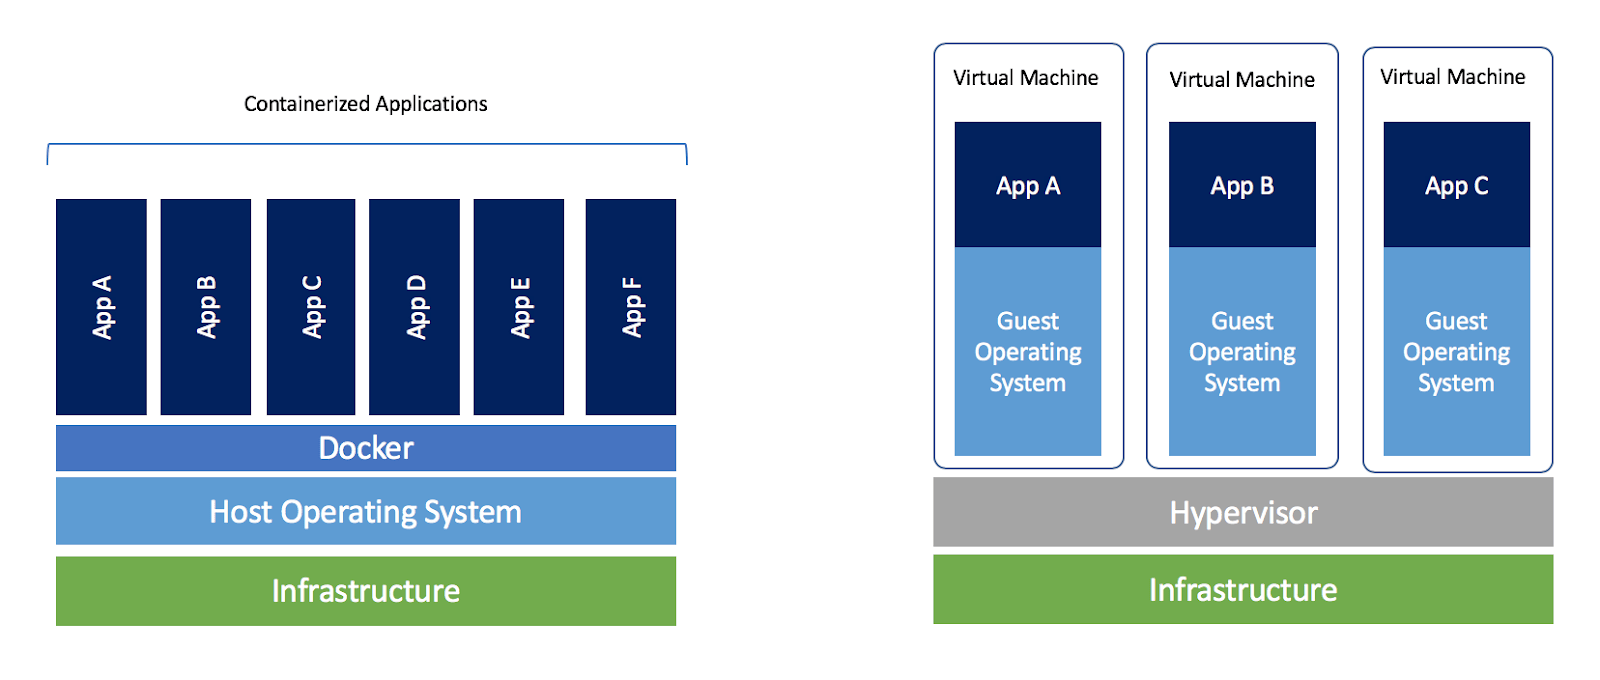
\includegraphics[width=0.6\columnwidth]{immagini/img/container_vs_vm} 
    \caption{Rappresentazione grafica dell'architettura a container ed a macchine virtuali}
\end{figure} \\
%TODO: immagine a layer raffgurante container vs virtual machine.
\\Un'architettura a \textbf{container} infatti, a differenza dell'architettura a macchine virtuali, garantisce un'esecuzione \textbf{separata} e \textbf{protetta} di \textbf{ogni singolo applicativo} compatibile con il sistema operativo host, indipendentemente dal numero di container presenti nel sistema o dal tipo di interfaccia di rete. \\
E' possibile, inoltre, far coesistere multipli container di uno stesso applicativo in esecuzione nello stesso momento (anche sfruttando il \textit{\gls{load-balancingg}}, come si accennerà nel corso di questa tesi) assegnandoci, esattamente come con le macchine virtuali, eventuali \textbf{indirizzi IP} statici, \textbf{CPU limit} e \textbf{disk quota}.\\
Essendo un container una \textbf{\gls{sandboxg}} applicativa indipendente dal sistema operativo, i dati generati dalla sua esecuzione sono destinati a scomparire nell'eventualità in cui il container venisse distrutto. Per ovviare a questo problema, si può ricorrere ad una tecnica di \textbf{volume-mapping}, ovvero una tecnica che permette di esporre il \textbf{\gls{filesystemg}} interno al container permettendone quindi la \textbf{lettura e scrittura} direttamente da parte dell'\textit{host}. La tecnica appena accennata sarà trattata in maniera più approfondita nel corso della lettura di questa tesi.\\
Godendo i container di un approccio standardizzato per la loro costruzione ed esecuzione, è quindi di facile intuizione la facilità di \textit{portabilità} di questi. Un container, infatti, può essere distribuito su una nuova piattaforma in maniera estremamente veloce e senza alcuna modifica allo stesso. Ne consegue, che un eventuale \textbf{rilascio e distribuzione} di un applicativo interno ad un container può essere molto velocizzato rispetto alla stessa operazione svolta invece su un'architettura a macchine virtuali. Relativamente sempre allo sviluppo e distribuzione di un applicativo, tramite container è possibile un controllo di versione dell'applicativo stesso più flessibile: è possibile infatti gestire le versioni del codice con le relative dipendenze inglobando il tutto in un unico container, formando quindi un'unità atomica di più facile manutenzione e distribuzione. Un eventuale ripristino o \textbf{\gls{rollbackg} delle modifiche potrà essere facilmente eseguito tramite \textbf{ripristino in esecuzione} del container contenente le modifiche precedentemente effettuate dal team.\\
Un altro dei vantaggi decisivi di un'architettura a container è la sua facilità di gestione. L'avvio, rimozione o la duplica dei container è un'operazione decisamente \textbf{meno onerosa} rispetto alla controparte nelle macchine virtuali (basti solo pensare al tempo di \textit{\gls{bootg}} del sistema operativo), e può essere \textbf{facilmente automatizzata e gestita} dal Docker Engine. Ne consegue quindi, che la \textbf{scalabilità}, ovvero la facilità di modifica dell'infrastruttura per far fronte alle variazioni di mole di informazioni trattate o carichi di lavoro, risulta di \textbf{gestione più semplice} anche per la figura sistemistica interna all'azienda.
\\
La presente immagine ritrae il browser web "Mozilla Firefox" in esecuzione all'interno di un container esposto all'\textit{host} nella porta 5800:
\begin{figure}[!h]     
\centering 
    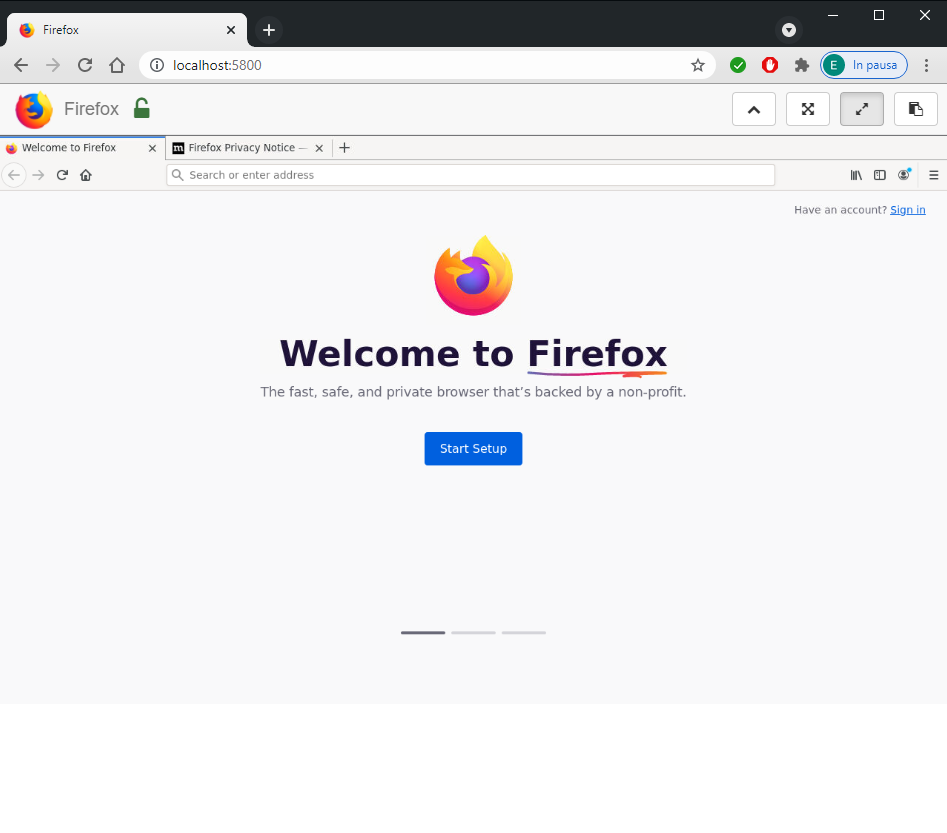
\includegraphics[width=0.6\columnwidth]{immagini/screenshot/firefox_container} 
    \caption{Browser web "Firefox" in esecuzione su un container con porta 5800 esposta all'host}
\end{figure} \\
%\begin{figure}[h!]
%    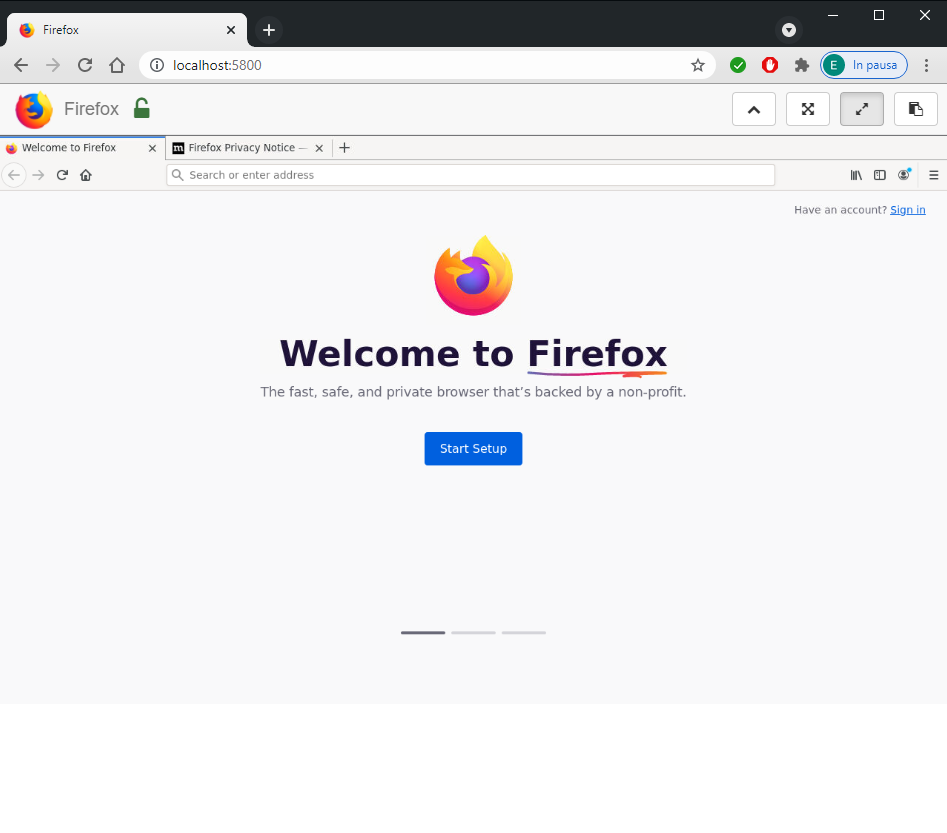
\includegraphics[width=1\textwidth]{./immagini/screenshot/firefox_container.png}
%    \caption{Applicativo "Firefox" in esecuzione su un container all'interno del browser web "Chrome"}
%\end{figure}
%TODO: come si ottiene un container (immagine s.o. + applicazione) vs come si ottiene lo stesso con una macchina virtuale.
\newpage
\section{Analisi di Docker: architettura e funzionalità}

Una delle piattaforme di riferimento più utilizzate e supportate in ambito container è appunto \textbf{Docker}. Nato dall'azienda dotCloud nel 2003 e pubblicato successivamente come progetto \textbf{\gls{open-sourceg}}, è una piattaforma atta alla gestione dei container. Tramite \textbf{Docker Desktop}\footcite{presente solamente per le versioni Windows}, è possibile monitorare, avviare, arrestare e gestire eventuali container creati. \\
Come già anticipato nel corso di questa tesi, Docker lavora a stretto contatto con il suo motore, ovvero \gls{Docker Engineg}, che si occupa appunto della \textbf{creazione} e \textbf{manutenzione} dei container nel sistema.
Il \textit{Docker Daemon} è il processo principale di Docker, cui compito è appunto la gestione e l'orchestrazione dei container nel sistema operativo dove è installato. \\
Al momento della creazione di un nuovo container, questo processo interroga i \textit{Docker Registries} per verificare la presenza di una immagine già pronta all'uso del programma che si vuole \textit{containerizzare}. I Docker Registries sono un insieme di immagini di container \textbf{pronte all'uso} e \textbf{scaricabili gratuitamente} da qualunque client Docker. Queste immagini sono create e manutenzionate dalla \textbf{Docker Community}, e permettono allo sviluppatore di avere delle immagini (o \textit{layer}) già pronti, testati e funzionanti al fine di costruire con successo la propria immagine di applicativo virtuale. Il Docker Registries più comune ed utilizzato è "\textbf{DockerHub}".\\
Come già menzionato nel corso di questo documento, tramite Docker è possibile costruire delle immagini di un applicativo virtuale. Un'immagine è un \textbf{set di comandi} cui scopo è quello di creare, una volta eseguito, un container. Un'immagine può basarsi, a sua volta, su altre immagini, ed il set di comandi che espandono l'immagine sorgente compongono, a loro volta, la nuova immagine applicativa. I comandi atti alla corretta costruzione della stessa vengono scritti su un apposito file, chiamato appunto "\textbf{dockerfile}", ed ogni comando (riga del file) si traduce in un nuovo \textit{layer} della nuova immagine. Un \textbf{dockerfile} è un documento di testo, senza alcuna estensione, contenente una serie di passi ed istruzioni atti alla \textbf{corretta creazione} di un' immagine di un applicativo. Il Docker Daemon, per costruire correttamente un' immagine, leggerà ed eseguirà in maniera \textbf{sequenziale} ogni comando trascritto all'interno del \textit{dockerfile}, ed al termine della lettura dello stesso, si avrà un'immagine eseguibile di un applicativo. \\
Un \textbf{container} è un'\textbf{istanza di esecuzione} di un'immagine a cui è attribuito un nome, arbitrario o definito dal programmatore, attraverso il Docker Daemon. 

%Tramite Docker è quindi possibile l'organizzazione e orchestrazione di tutti i container applicativi installati sul client.


\section{Creazione di container vs creazione di VM}

La creazione di una VM è possibile tramite apposito \textit{hypervisor}. Tuttavia, al momento della creazione, l'utente deve essere a conoscenza della quantità massima di risorse \textit{hardware} da destinare alla stessa. Questa stima, oltre ad includere il costo\footcite{inteso come quantitativo di risorse fisiche da allocare} richiesto dal programma da \textit{virtualizzare} che si andrà ad installare all'interno della VM, deve includere anche il costo, almeno soddisfacente i requisiti minimi, relativo al sistema operativo. 
%La seguente schermata rappresenta la creazione della macchina virtuale con 8Gb di RAM e 80Gb di disco rigido dedicati:\\
%TODO: immagine di avvio dell'installazione di Windows 10 Pro da VMWARE
Terminata la fase di \textbf{analisi dei costi}, sarà necessario installare \textbf{manualmente} il sistema operativo all'interno della macchina virtuale appena creata. Per fare ciò, bisognerà avviare la macchina virtuale da un supporto di \textbf{boot}, come ad esempio una immagine \gls{ISOg} avviabile di un sistema operativo.
Successivamente alla fase di avvio di installazione della VM, si passerà alla fase vera e propria di installazione del sistema operativo.\\%, riassunta nelle seguenti immagini:
%TODO: immagini dell'installazione del sistema operativo nella VM con VMWARE.
Una volta ottenuta un'installazione funzionante ed avviabile, per ottimizzarne al meglio le prestazioni, tramite ad esempio installazione dei relativi \gls{driverg} video virtuali, ed espanderne le funzionalità, come la possibilità di accedere a \textit{volume-mapping} condivisi con il sistema operativo \textit{host}, è necessario installare le relative \textbf{\gls{guest additionsg}}, proprie di ciascun programma di virtualizzazione.
%TODO: immagine raffigurante l'installazione delle Guest Additions su VMWARE.
Una volta fatti i passi sopra-descritti, si avrà un sistema operativo virtualizzato completamente funzionante, pronto per l'installazione di tutto il software applicativo desiderato.
%TODO: immagine raffigurante W10 Pro avviato e funzionante con Firefox in esecuzione.
\\
Come precedentemente affermato, un container è un'unità atomica costituita principalmente da una o più applicazioni e dalle librerie di sistema operativo atte al loro corretto funzionamento.
Al fine di poter generare ed utilizzare prima un'immagine applicativa e successivamente un container, è necessario prima costruirne il relativo \textbf{\gls{dockerfileg}}.
Ogni \textit{dockerfile} di ogni immagine applicativa contiene un set di istruzioni e comandi atti alla corretta installazione e configurazione dell'applicativo virtuale. Ogni comando scritto nel \textit{dockerfile} comporrà un nuovo \textit{layer} del container.
%Le seguenti immagini mostrano i corretti passi per la costruzione di un container con, all'interno, l'applicativo "Firefox":
%TODO: immagini raffiguranti i passi e comandi atti alla creazione di un container
La creazione di multipli container cloni, ovvero container generati da una singola immagine, è un'operazione di semplice e veloce esecuzione, in quanto il Docker Engine, durante la costruzione di ogni container, adotta un meccanismo di \textit{\gls{cachingg}} dei vari \textit{\gls{layerg}} di cui un container è composto. Questo meccanismo permette quindi una costruzione, o aggiornamento, di un container \textbf{molto più veloce} rispetto ad una sua completa ri-creazione, in quanto si useranno, se compatibili, i layer in cache già \textbf{precedentemente costruiti} al fine di costruire il nuovo container contenente l'applicativo, nuovo o aggiornato, desiderato.\\
Durante tutta la durata dello stage si è utilizzata la piattaforma "Docker" per la creazione delle varie immagini e container per gli applicativi specificati nel sommario e nell'introduzione.

\section{Installazione di Docker in ambiente Windows}
Al fine di poter creare ed orchestrare dei container, è necessaria l'installazione del software "\textbf{Docker Desktop}" nel proprio computer. Docker Desktop è compatibile con tutte le versioni di Windows a partire da Windows 10 Home (build 19041), ed i requisiti minimi sono i seguenti:
\begin{itemize}
	\item Processore a \textbf{64 bit};
	\item 4Gb di memoria \textbf{RAM};
	\item Virtualizzazione hardware abilitata da \textbf{\gls{BIOSg}};
	\item Funzionalità \textbf{Hyper-V} abilitata da Windows.
\end{itemize}
\textbf{N.B:} per abilitare il supporto di virtualizzazione Hyper-V su Windows bastera' accedere all'apposito menu "\textbf{Abilita o disabilita funzionalità di Windows}" e selezionare la voce "\textbf{Hyper-V}".
\\
%TODO: immagine mostrante l'abilitazione della funzionalità Hyper-V su Windows.
Una volta scaricato l'\gls{installerg} di Docker Desktop, l'installazione è una procedura relativamente semplice, in quanto è del tipo "\textbf{one click-install}".\\
Durante tutta l'installazione è necessaria una connessione ad internet attiva.\\
Terminata l'installazione, per avviare Docker Desktop basterà aprire il menu \textbf{Start} di Windows e cliccare sulla relativa icona di Docker Desktop come nell'immagine:\\
\begin{figure}[!h]     
\centering 
    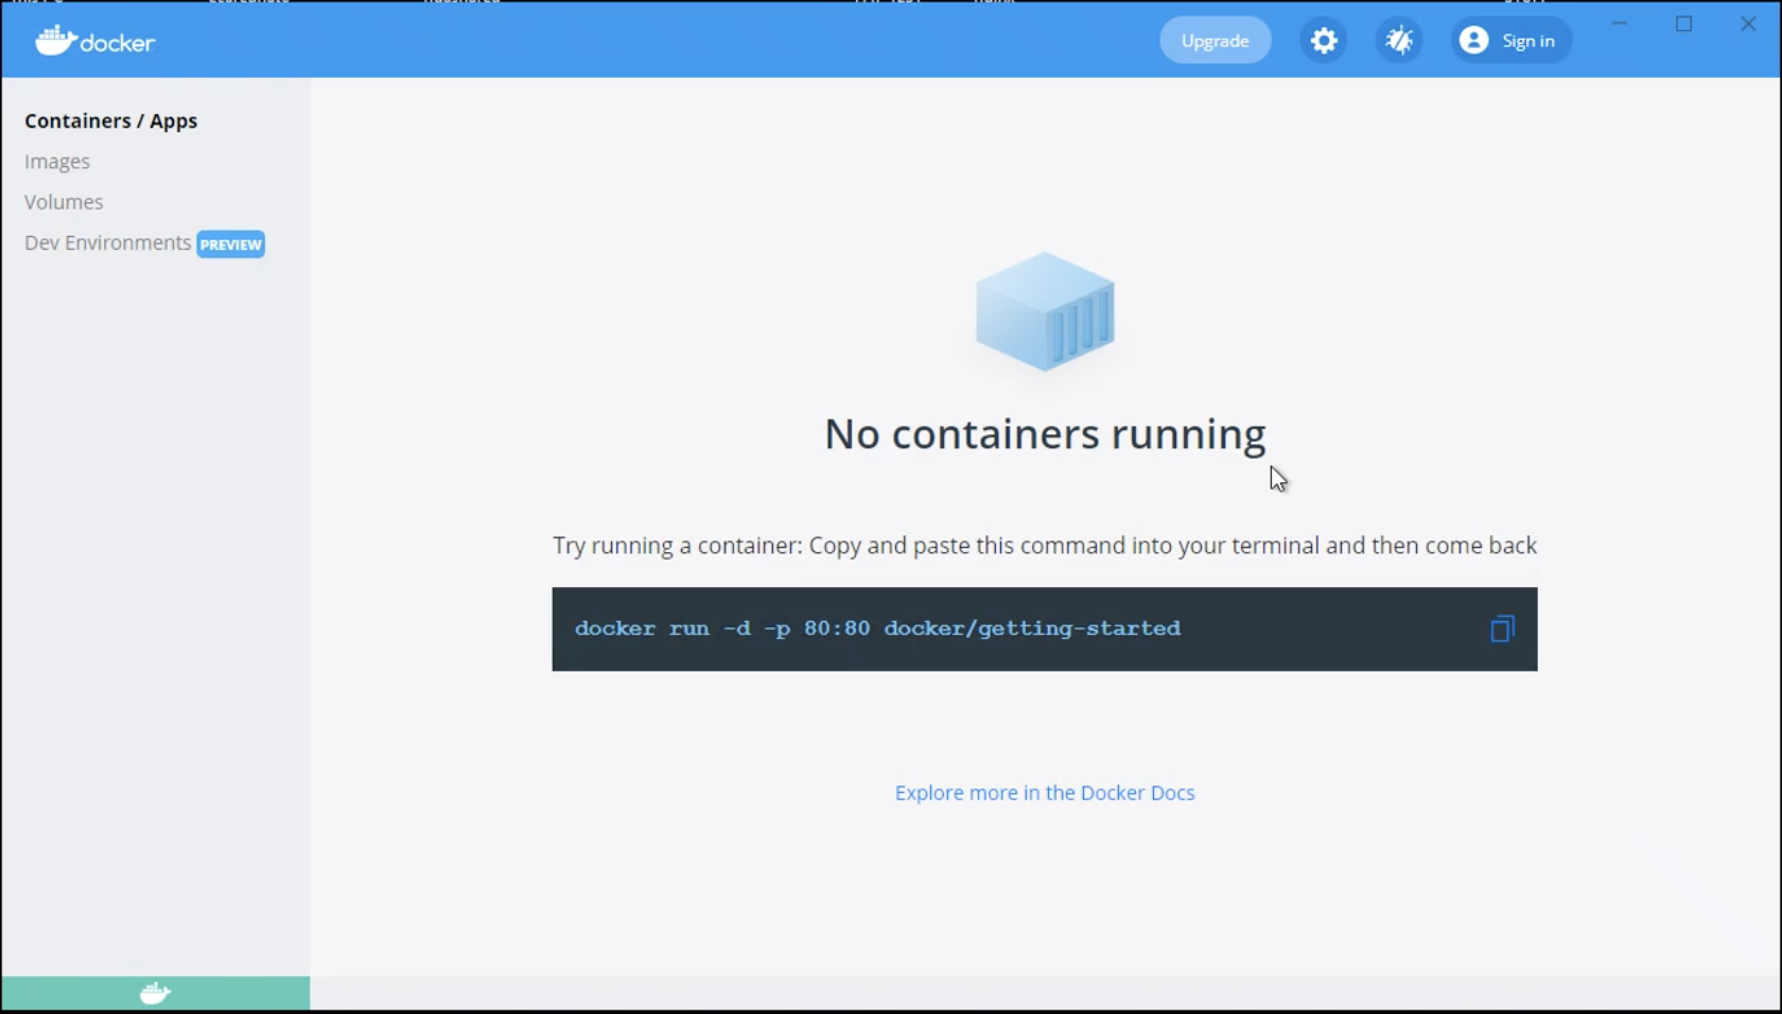
\includegraphics[width=1.0\columnwidth]{immagini/screenshot/docker_desktop_initialscreen} 
    \caption{Schermata principale di "Docker Desktop" con nessun container in esecuzione}
\end{figure} \\

%TODO: immagine mostrante l'icona di Docker Desktop presente nel menu Start di Windows terminata l'installazione.

